\documentclass[14pt]{beamer}
\usepackage{fontspec}
\usepackage{mathtools}
\usetheme[progressbar=head]{metropolis}          
\setsansfont[BoldFont={Fira Sans SemiBold}]{Fira Sans Book}
\title{Underwater Real-Time Object Recognition and Tracking for Autonomous Underwater Vehicle}
\author{Tan Soon Jin}
\date{\today}
\institute{National University of Singapore}
\begin{document}
\maketitle

%%%%%%%%%%%%%%%%%%%%%%%%%%%%%%%%%%%%%%%%%%%%%%%%%%%%%%%%%%%%%%%%%%%%%%%%%%%%%%%%%%%%%%%%%%%%%%%%%%%%

\section{Background}


\begin{frame}{AUV (Autonomous Underwater Vehicle)}

  \begin{figure}[ht]
      \centering
      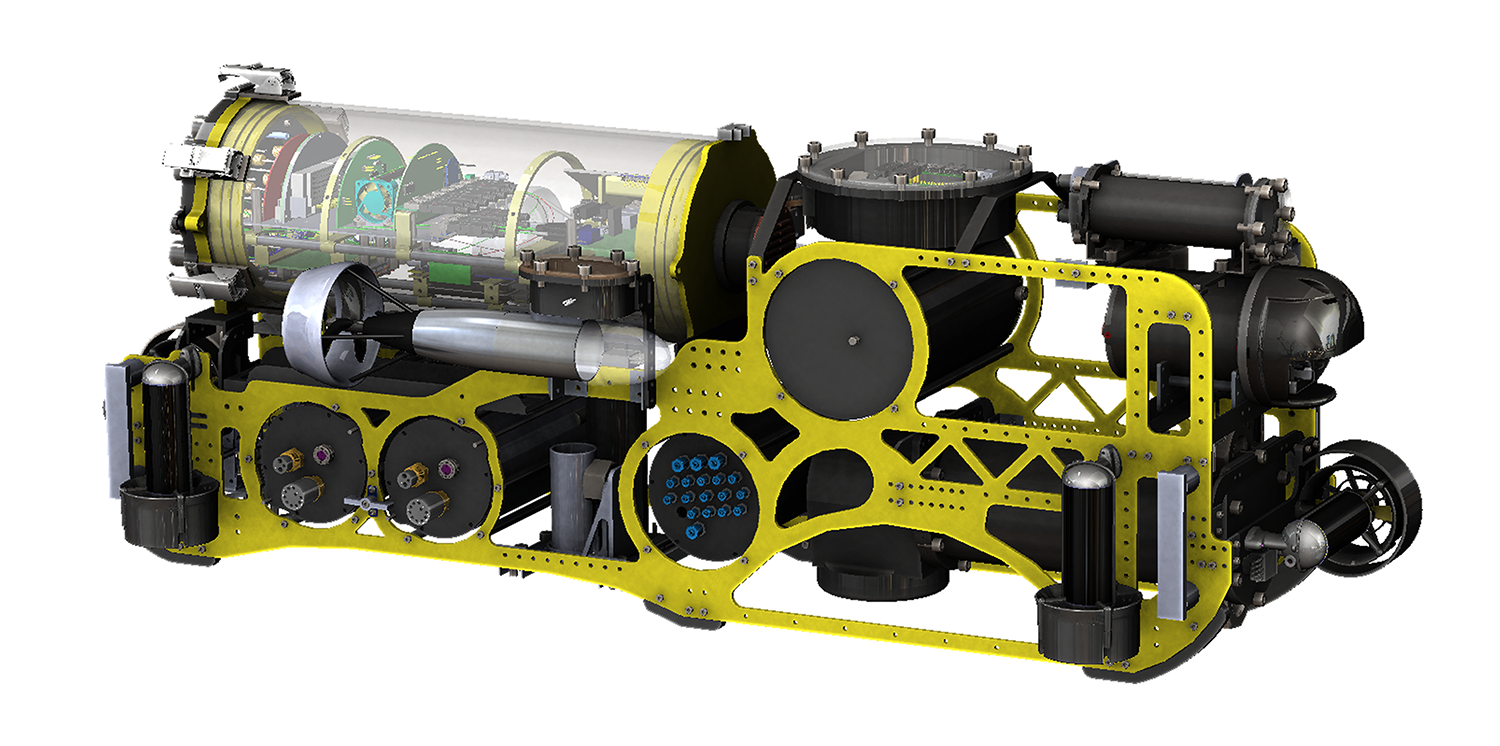
\includegraphics[width=0.5\textwidth, height=0.3\textwidth]{figs/auv.png}
  \end{figure}

  \textbf{AUV} is a robot that travels underwater without requiring input from an operator.

\end{frame}

\begin{frame}{Some applications of AUV}

  \begin{figure}[ht]
      \centering
      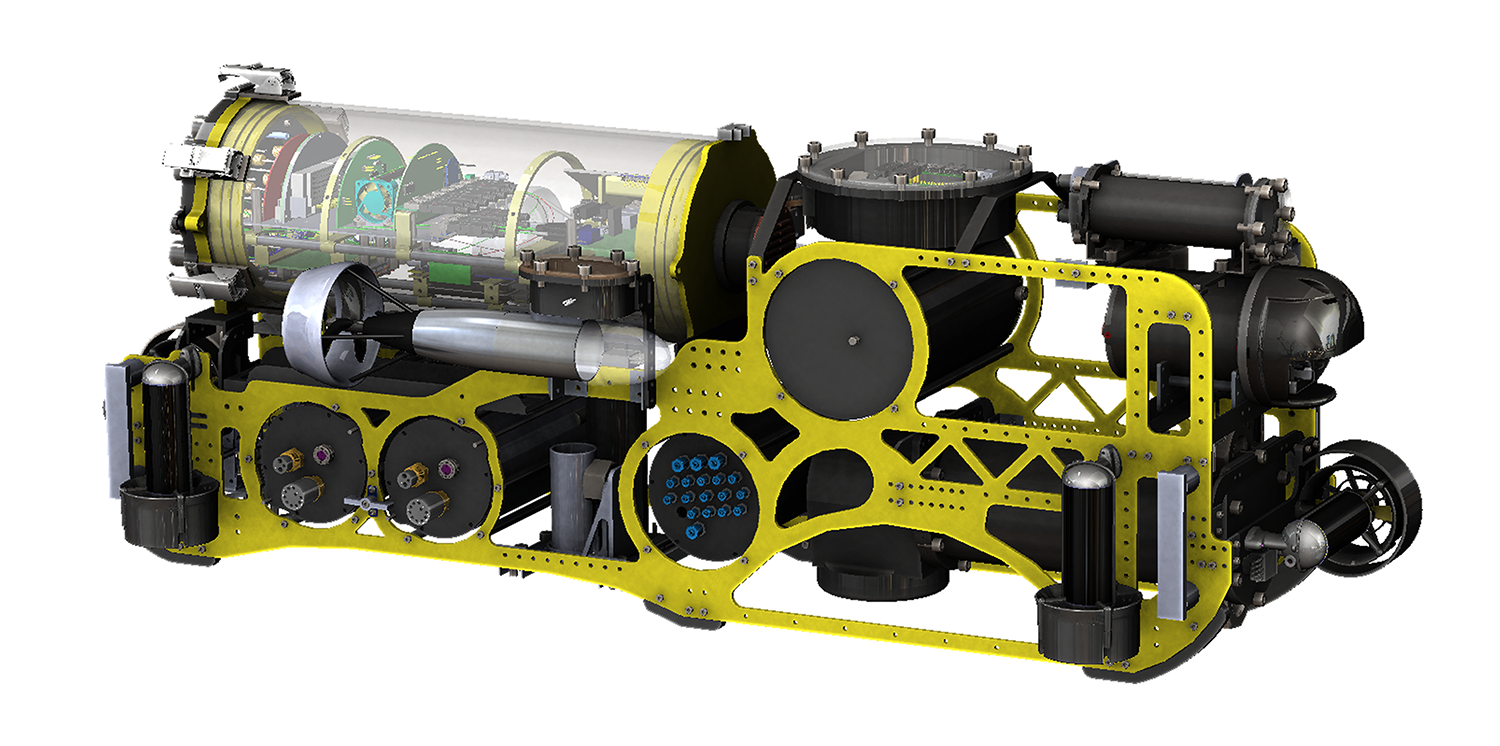
\includegraphics[width=0.5\textwidth, height=0.3\textwidth]{figs/auv.png}
  \end{figure}

  \begin{enumerate}
    \item Air crash investigation
    \item Conduct research on life of marine organisms
    \item Make detailed maps of the seafloor
  \end{enumerate}

\end{frame}

\begin{frame}{Robosub}

  \begin{figure}[ht]
      \centering
      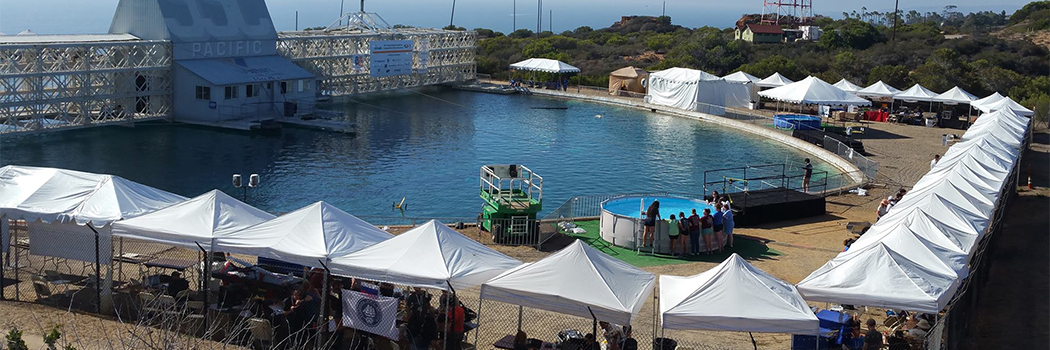
\includegraphics[width=0.5\textwidth, height=0.3\textwidth]{figs/robosub.jpg}
  \end{figure}

  \textbf{Robosub} is an international AUV competition held annually in San Diego.

\end{frame}

\begin{frame}{Visual-based tasks}

  \begin{figure}[ht]
      \centering
      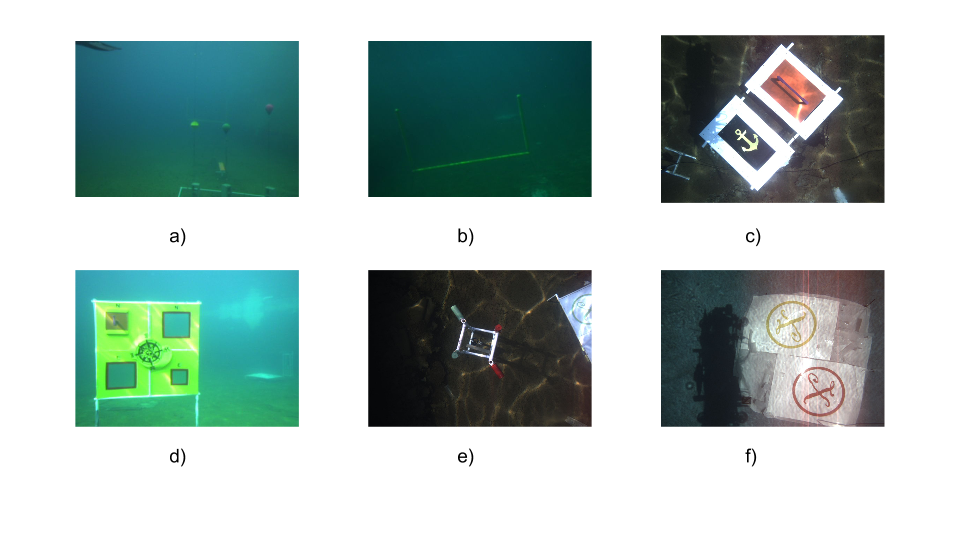
\includegraphics[width=0.6\textwidth, height=0.4\textwidth]{figs/tasks.png}
  \end{figure}

  Each AUV is required to complete a series of visual-based tasks that simulate
  the actual work of an AUV.

\end{frame}
%%%%%%%%%%%%%%%%%%%%%%%%%%%%%%%%%%%%%%%%%%%%%%%%%%%%%%%%%%%%%%%%%%%%%%%%%%%%%%%%%%%%%%%%%%%%%%%%%%%%

\begin{frame}[standout]{}
  Design a robust underwater vision framework for AUV to complete visual tasks
  in Robosub
\end{frame}
%%%%%%%%%%%%%%%%%%%%%%%%%%%%%%%%%%%%%%%%%%%%%%%%%%%%%%%%%%%%%%%%%%%%%%%%%%%%%%%%%%%%%%%%%%%%%%%%%%%%

\section{Motivation}

\begin{frame}{Problem 1: Underwater vision challenges}

  \begin{figure}[ht]
      \centering
      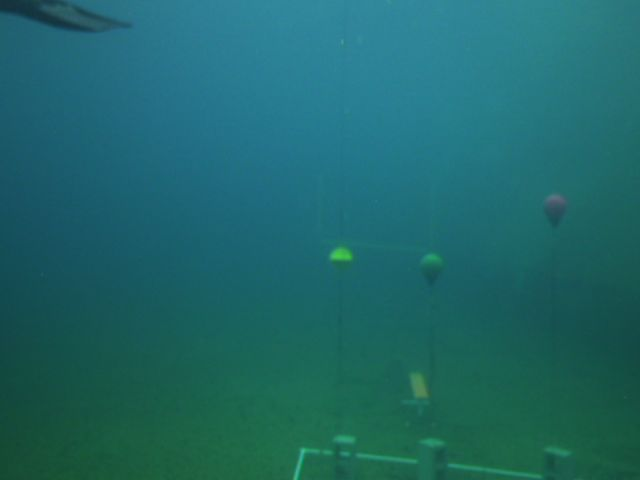
\includegraphics[width=0.5\textwidth, height=0.3\textwidth]{figs/problem1_1.png}
  \end{figure}

  Can you identify the {\color{red} \textbf{RED}} buoy ? 

\end{frame}

\begin{frame}{Problem 1: Underwater vision challenges}

  \begin{figure}[ht]
      \centering
      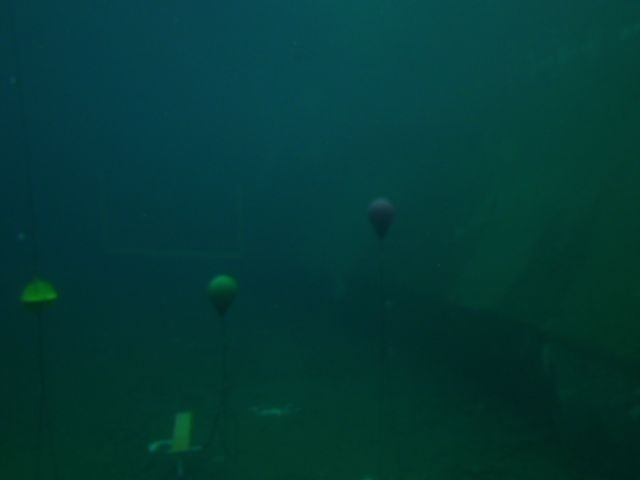
\includegraphics[width=0.5\textwidth, height=0.3\textwidth]{figs/problem1_2.jpg}
  \end{figure}

  Can you still identify the {\color{red} \textbf{RED}} buoy ? 

\end{frame}

\begin{frame}{Problem 1: Underwater vision challenges}

    \begin{figure}
        \centering
        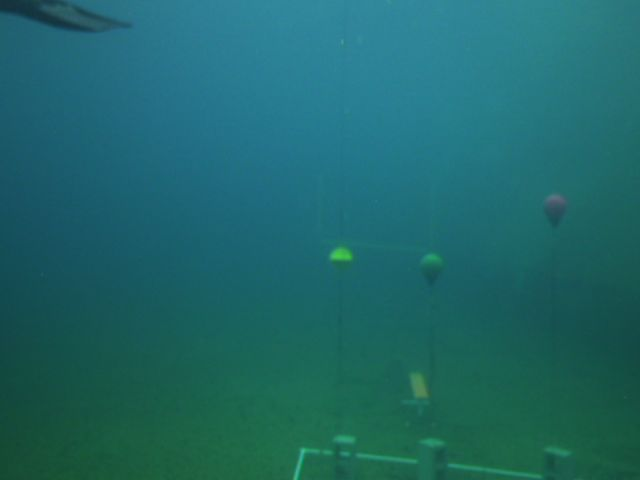
\includegraphics[width=0.4\textwidth, height=0.3\textheight]{figs/problem1_1.png}\hspace{2em}
        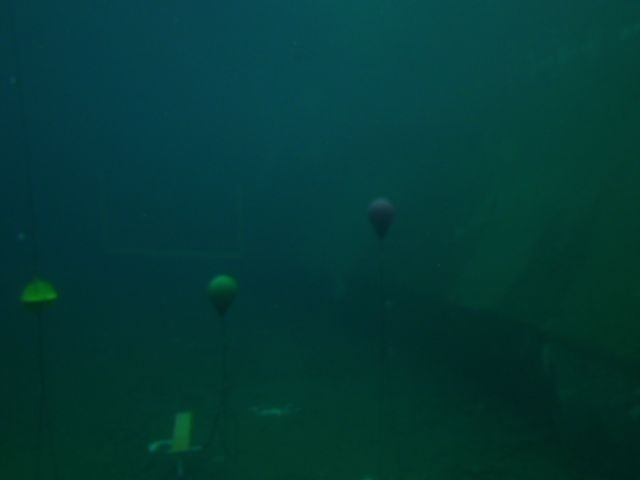
\includegraphics[width=0.4\textwidth, height=0.3\textheight]{figs/problem1_2.jpg}
    \end{figure}

  How do we \textbf{consistently} identify an object underwater ?

\end{frame}

\begin{frame}{Problem 2: Time constraint}

  \begin{figure}[ht]
      \centering
      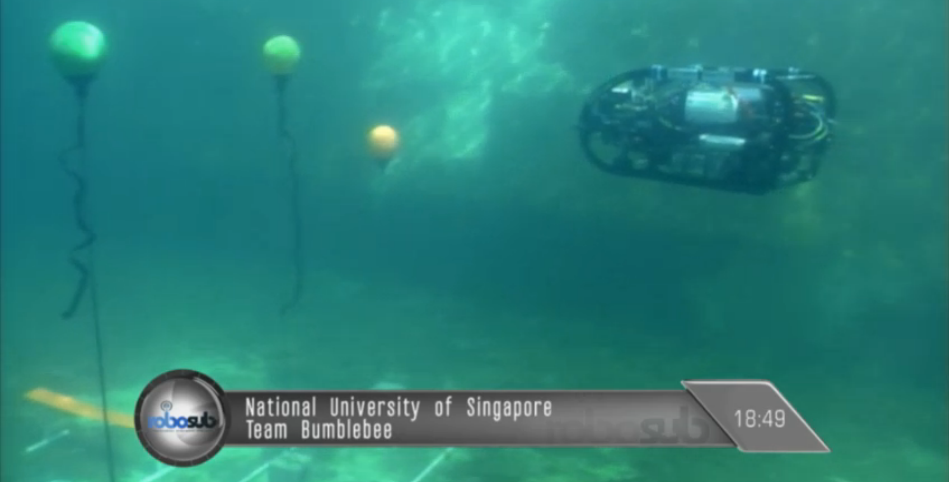
\includegraphics[width=0.5\textwidth, height=0.3\textwidth]{figs/problem2_1.png}
  \end{figure}

  \begin{enumerate}
    \item Low detection latency
    \item Limited amount of data
  \end{enumerate}

\end{frame}
%%%%%%%%%%%%%%%%%%%%%%%%%%%%%%%%%%%%%%%%%%%%%%%%%%%%%%%%%%%%%%%%%%%%%%%%%%%%%%%%%%%%%%%%%%%%%%%%%%%%

\begin{frame}[standout]{}
  \begin{enumerate}
    \item Preprocessing
    \item Object Proposals
    \item Feature Design
  \end{enumerate}
\end{frame}
%%%%%%%%%%%%%%%%%%%%%%%%%%%%%%%%%%%%%%%%%%%%%%%%%%%%%%%%%%%%%%%%%%%%%%%%%%%%%%%%%%%%%%%%%%%%%%%%%%%%

\section{Preprocessing}

\begin{frame}{Color Correction: Methodology}
  \begin{enumerate}
    \item Estimating the true illuminants based on certain assumptions i.e
      (Grey-World, White Patch)
    \item Image correction using von Kries transformation
      \[
      \begin{pmatrix}
        R_c \\
        G_c \\
        B_c \\
      \end{pmatrix}
      =
      \begin{pmatrix}
        d_1 & 0 & 0 \\
        0 & d_2 & 0 \\
        0 & 0 & d_3\\
      \end{pmatrix}
      \begin{pmatrix}
        R_u \\
        G_u \\
        B_u \\
      \end{pmatrix}
      \]
  \end{enumerate}
\end{frame}

\begin{frame}{Color Correction: Results}

  \begin{figure}[ht]
      \centering
      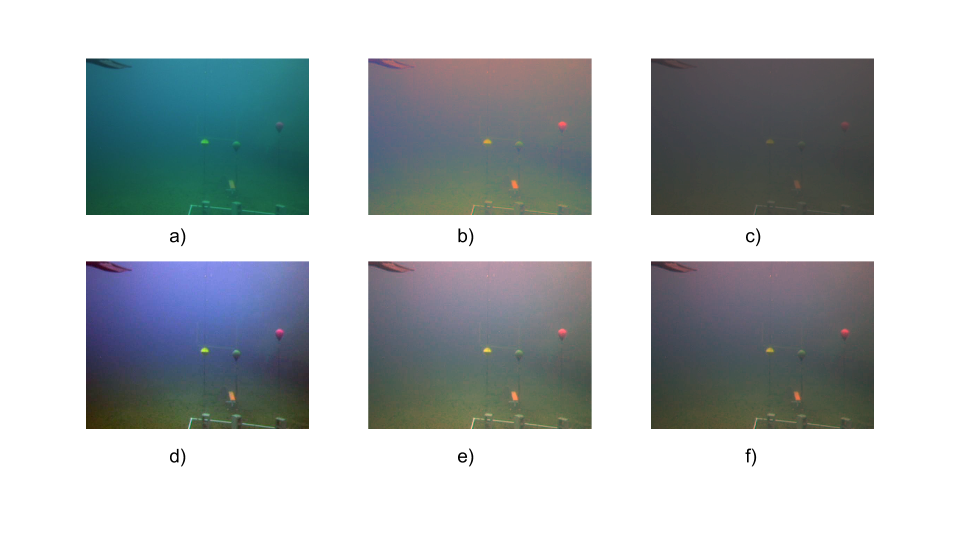
\includegraphics[width=0.9\textwidth, height=0.6\textwidth]{figs/color_constancy.png}
  \end{figure}

\end{frame}

\begin{frame}{Fusion-based enhancement: Overview}

  \begin{figure}[ht]
      \centering
      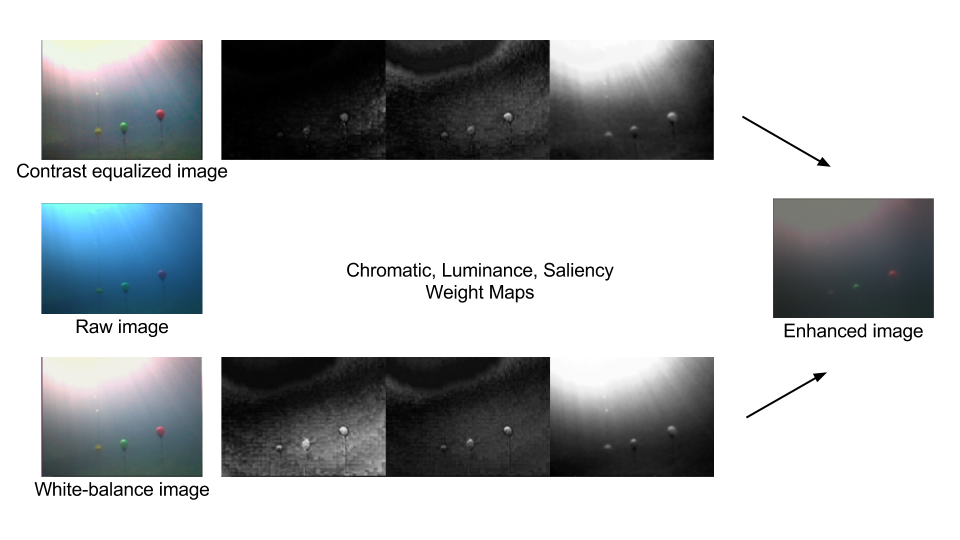
\includegraphics[width=0.9\textwidth, height=0.6\textwidth]{figs/fusion_pipeline.png}
  \end{figure}

\end{frame}

\begin{frame}{Methodology: Preprocess input}
  \begin{enumerate}
    \item Compute color corrected image as \textbf{\textit{input1}}
    \item Compute contrast enhanced \textit{input1} as \textbf{\textit{input2}}
  \end{enumerate}
\end{frame}

\begin{frame}{Methodology: Compute weight maps}

  \begin{figure}[ht]
      \centering
      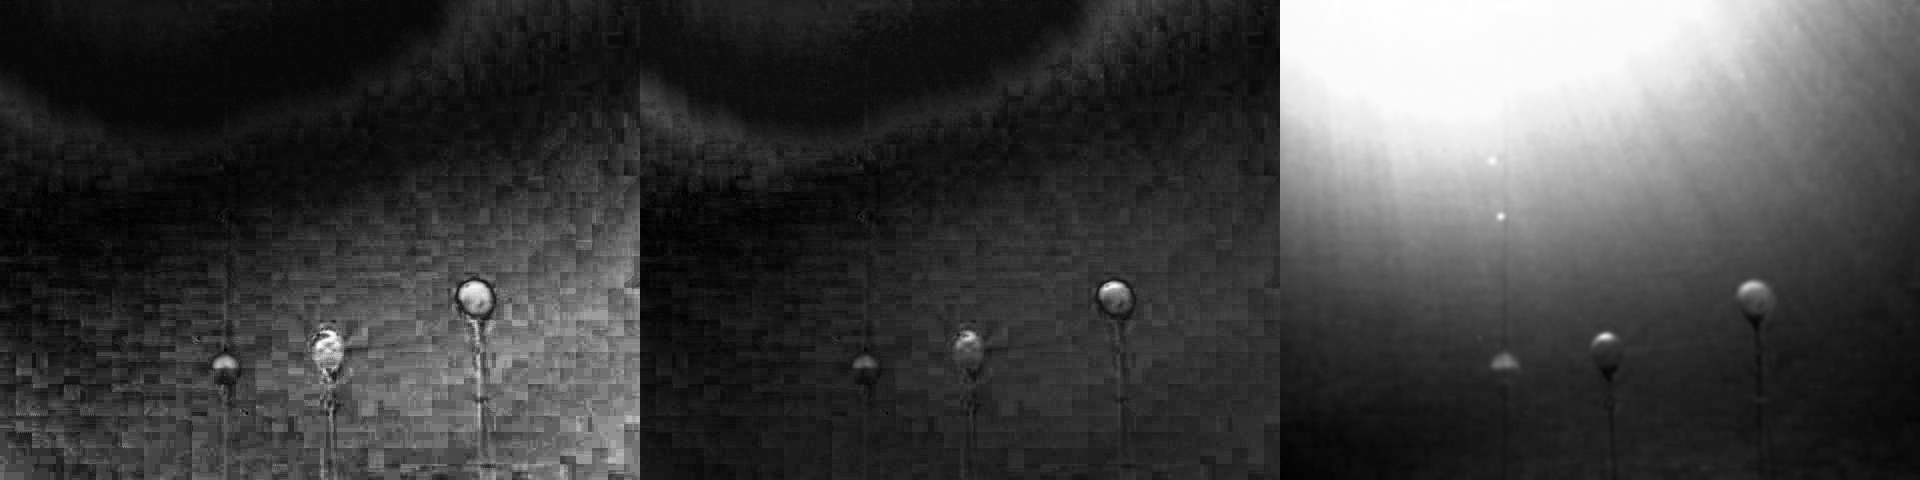
\includegraphics[width=0.5\textwidth, height=0.2\textwidth]{figs/weightmaps.png}
      \caption{Weight maps (left to right): chromatic map, luminance map,
        saliency map}
  \end{figure}

  \begin{enumerate}
    \item Compute weight maps for \textit{input1} and \textit{input2}
    \item Normalize the 2 sets of weight maps
  \end{enumerate}
\end{frame}

\begin{frame}{Methodology: Pyramid-based image fusion}

  \begin{figure}[ht]
      \centering
      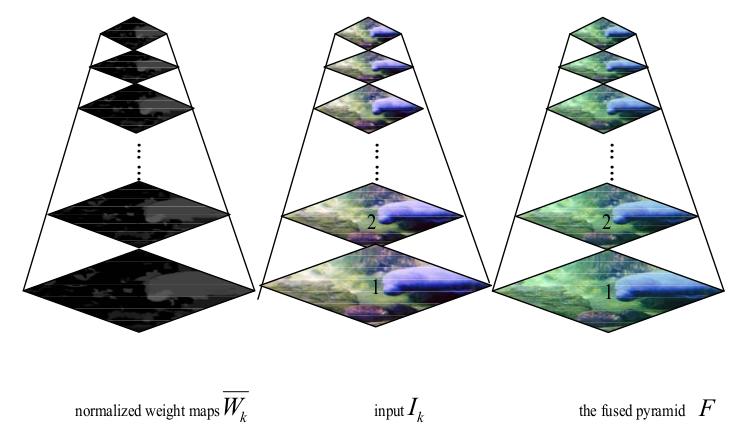
\includegraphics[width=0.8\textwidth, height=0.4\textwidth]{figs/pyramid.png}
  \end{figure}

  \begin{enumerate}
    \item Generates image pyramid for each inputs and weight maps
    \item Fuse the normalized weight maps with input  using the generated pyramids
  \end{enumerate}
\end{frame}

\begin{frame}{Image denoising: Homomorphic filter}

  \begin{figure}[ht]
      \centering
      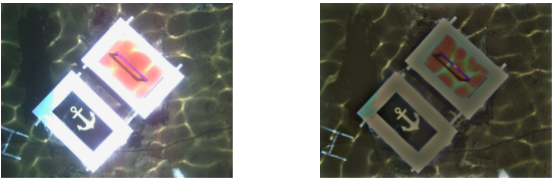
\includegraphics[width=0.6\textwidth, height=0.3\textwidth]{figs/homomorphic.png}
  \end{figure}

  \textbf{Homomorphic filter} removes multiplicative noise by applying high-pass
  filter on the image.

\end{frame}

\begin{frame}{Illumination Compensation}

  \begin{figure}[ht]
      \centering
      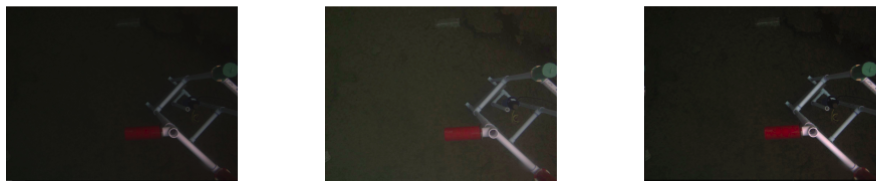
\includegraphics[width=0.8\textwidth, height=0.3\textwidth]{figs/illumination_compensation.png}
  \end{figure}

  \begin{enumerate}
    \item Gamma-based correction
    \item Log-based correction
  \end{enumerate}
\end{frame}
%%%%%%%%%%%%%%%%%%%%%%%%%%%%%%%%%%%%%%%%%%%%%%%%%%%%%%%%%%%%%%%%%%%%%%%%%%%%%%%%%%%%%%%%%%%%%%%%%%%%

\section{Object Proposals}

\begin{frame}{How it used to work: Sliding window}

  \begin{figure}[ht]
      \centering
      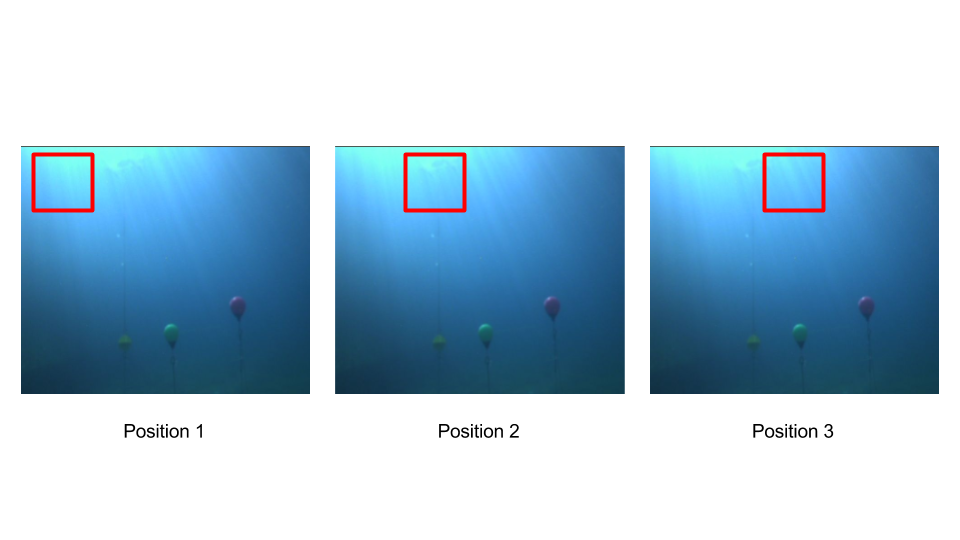
\includegraphics[width=0.7\textwidth, height=0.4\textwidth]{figs/sliding_window.png}
  \end{figure}

  High-detection latency if multiscale-detection is required and detection dependent solely
  on object classifier.
\end{frame}

\begin{frame}{New approach: Object proposals}

  \begin{figure}[ht]
      \centering
      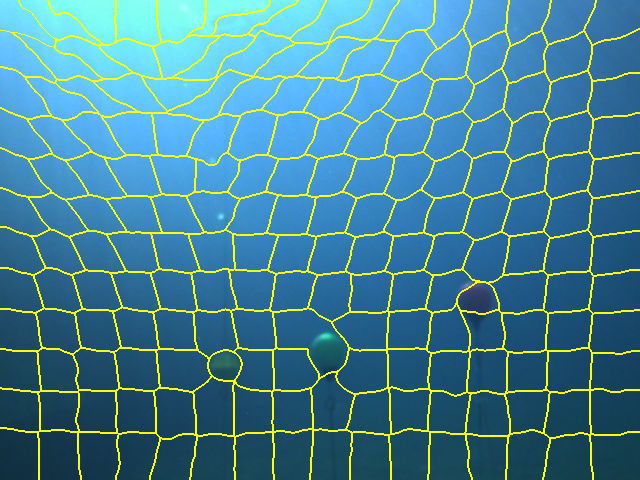
\includegraphics[width=0.5\textwidth, height=0.3\textwidth]{figs/slic.png}
      \caption{Superpixel-based segmentation}
  \end{figure}

  Generates candidate window based on segmentation of the image. Group segments
  with similar properties such as color cue.
\end{frame}

\begin{frame}{Role of object proposals}

  \begin{enumerate}
    \item A more general object detector using cues like edges and color
    \item Prevent false negatives because of strict object classifiers
  \end{enumerate}
\end{frame}

\begin{frame}{Selective Search}

  \begin{figure}[ht]
      \centering
      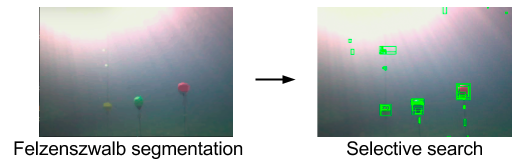
\includegraphics[width=0.8\textwidth, height=0.4\textwidth]{figs/selectivesearch.png}
  \end{figure}

  \begin{enumerate}
    \item Perform graph-cut based segmentations
    \item Hierarchical grouping of similar segments
  \end{enumerate}
\end{frame}

\begin{frame}{MSER (Maximally Stable Extremal Regions)}

  \begin{figure}[ht]
      \centering
      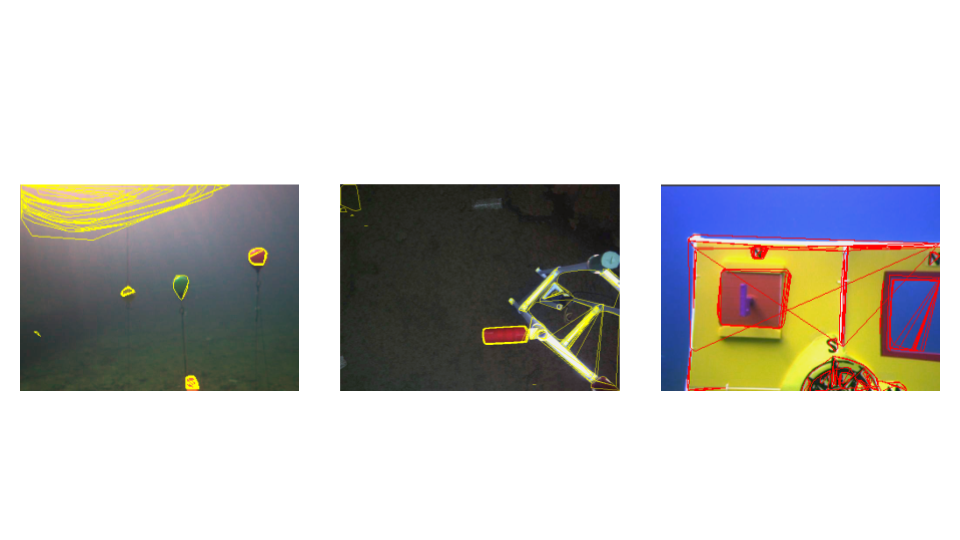
\includegraphics[width=0.8\textwidth, height=0.5\textwidth]{figs/mserproposal.png}
  \end{figure}

  {\small Detects regions that remain stable over different thresholds applied
    on the input image.}
\end{frame}

\begin{frame}{Saliency}

  \begin{figure}[ht]
      \centering
      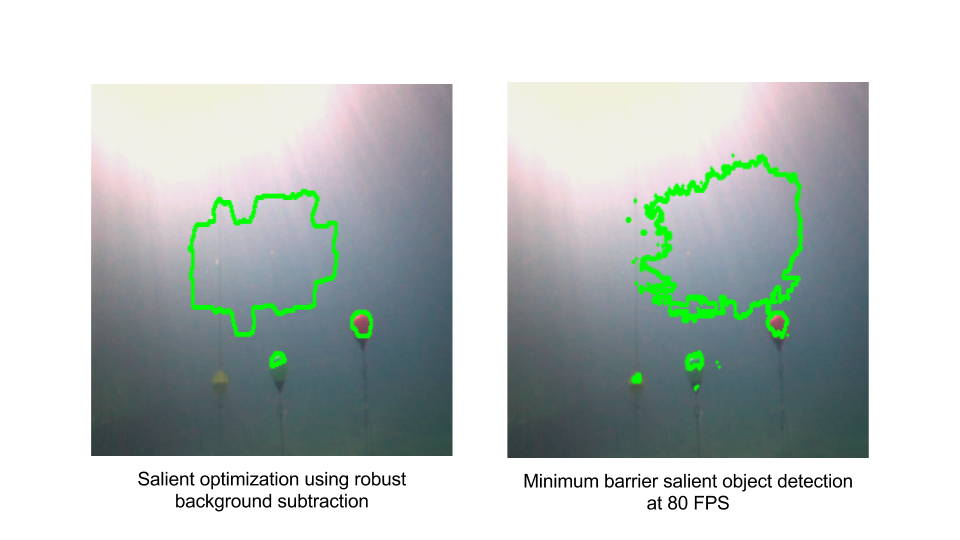
\includegraphics[width=0.7\textwidth, height=0.4\textwidth]{figs/saliency.png}
  \end{figure}

  {\small This approach labels regions that pop-out in the human visual system.
    Surprisingly powerful for detecting objects in the competition}
\end{frame}
%%%%%%%%%%%%%%%%%%%%%%%%%%%%%%%%%%%%%%%%%%%%%%%%%%%%%%%%%%%%%%%%%%%%%%%%%%%%%%%%%%%%%%%%%%%%%%%%%%%%

\section{Feature Design}

\begin{frame}{Datasets: Part 1}
  \begin{figure}[ht]
      \centering
      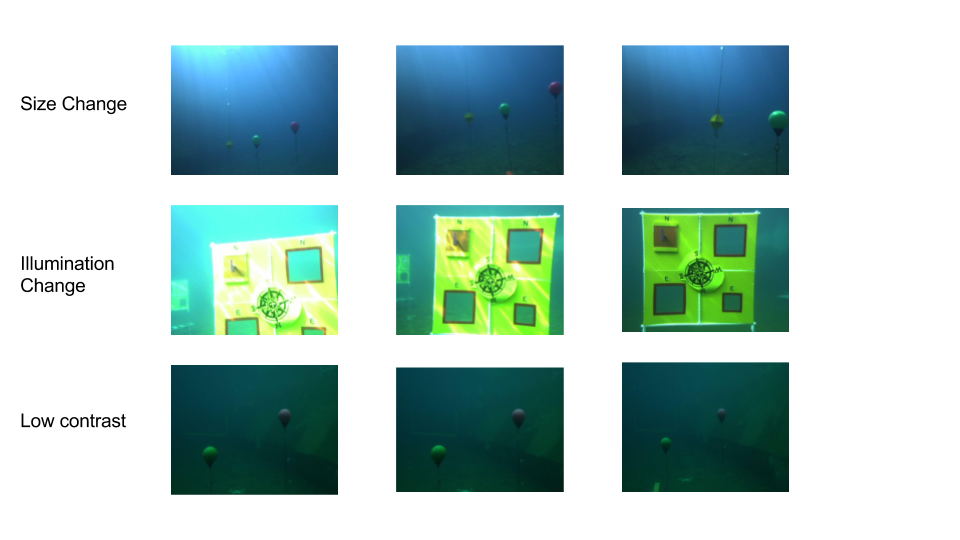
\includegraphics[width=0.9\textwidth, height=0.6\textwidth]{figs/data1.png}
  \end{figure}
\end{frame}

\begin{frame}{Datasets: Part 2}
  \begin{figure}[ht]
      \centering
      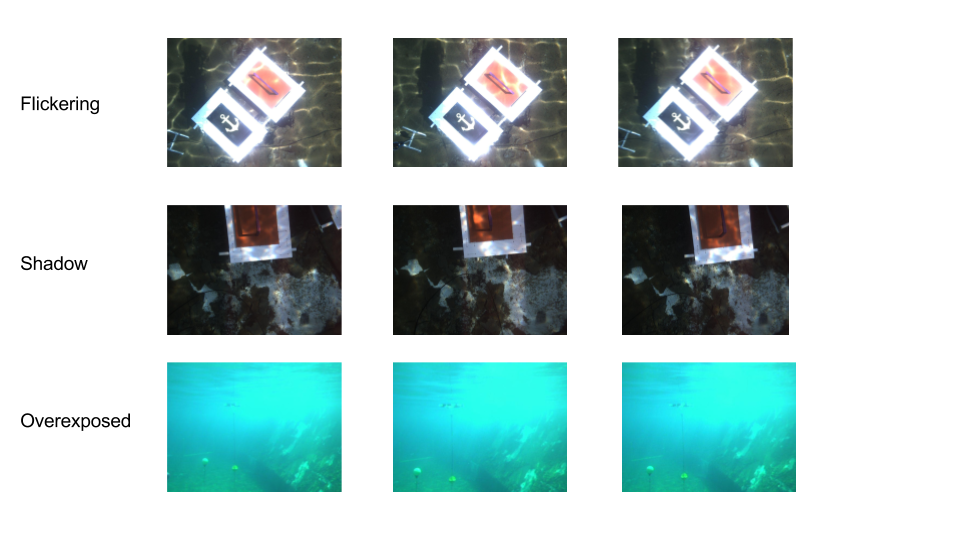
\includegraphics[width=0.9\textwidth, height=0.6\textwidth]{figs/data2.png}
  \end{figure}
\end{frame}

\begin{frame}{Requirements}
  To achieve a consistent object tracking under different sets of challenges,
  the features used for training needs to achieve certain degree of invariance.
  \begin{enumerate}
    \item Illumination invariance
    \item Scale \& rotation invariance
  \end{enumerate}
\end{frame}

\begin{frame}{Color descriptors}

  \begin{figure}[ht]
      \centering
      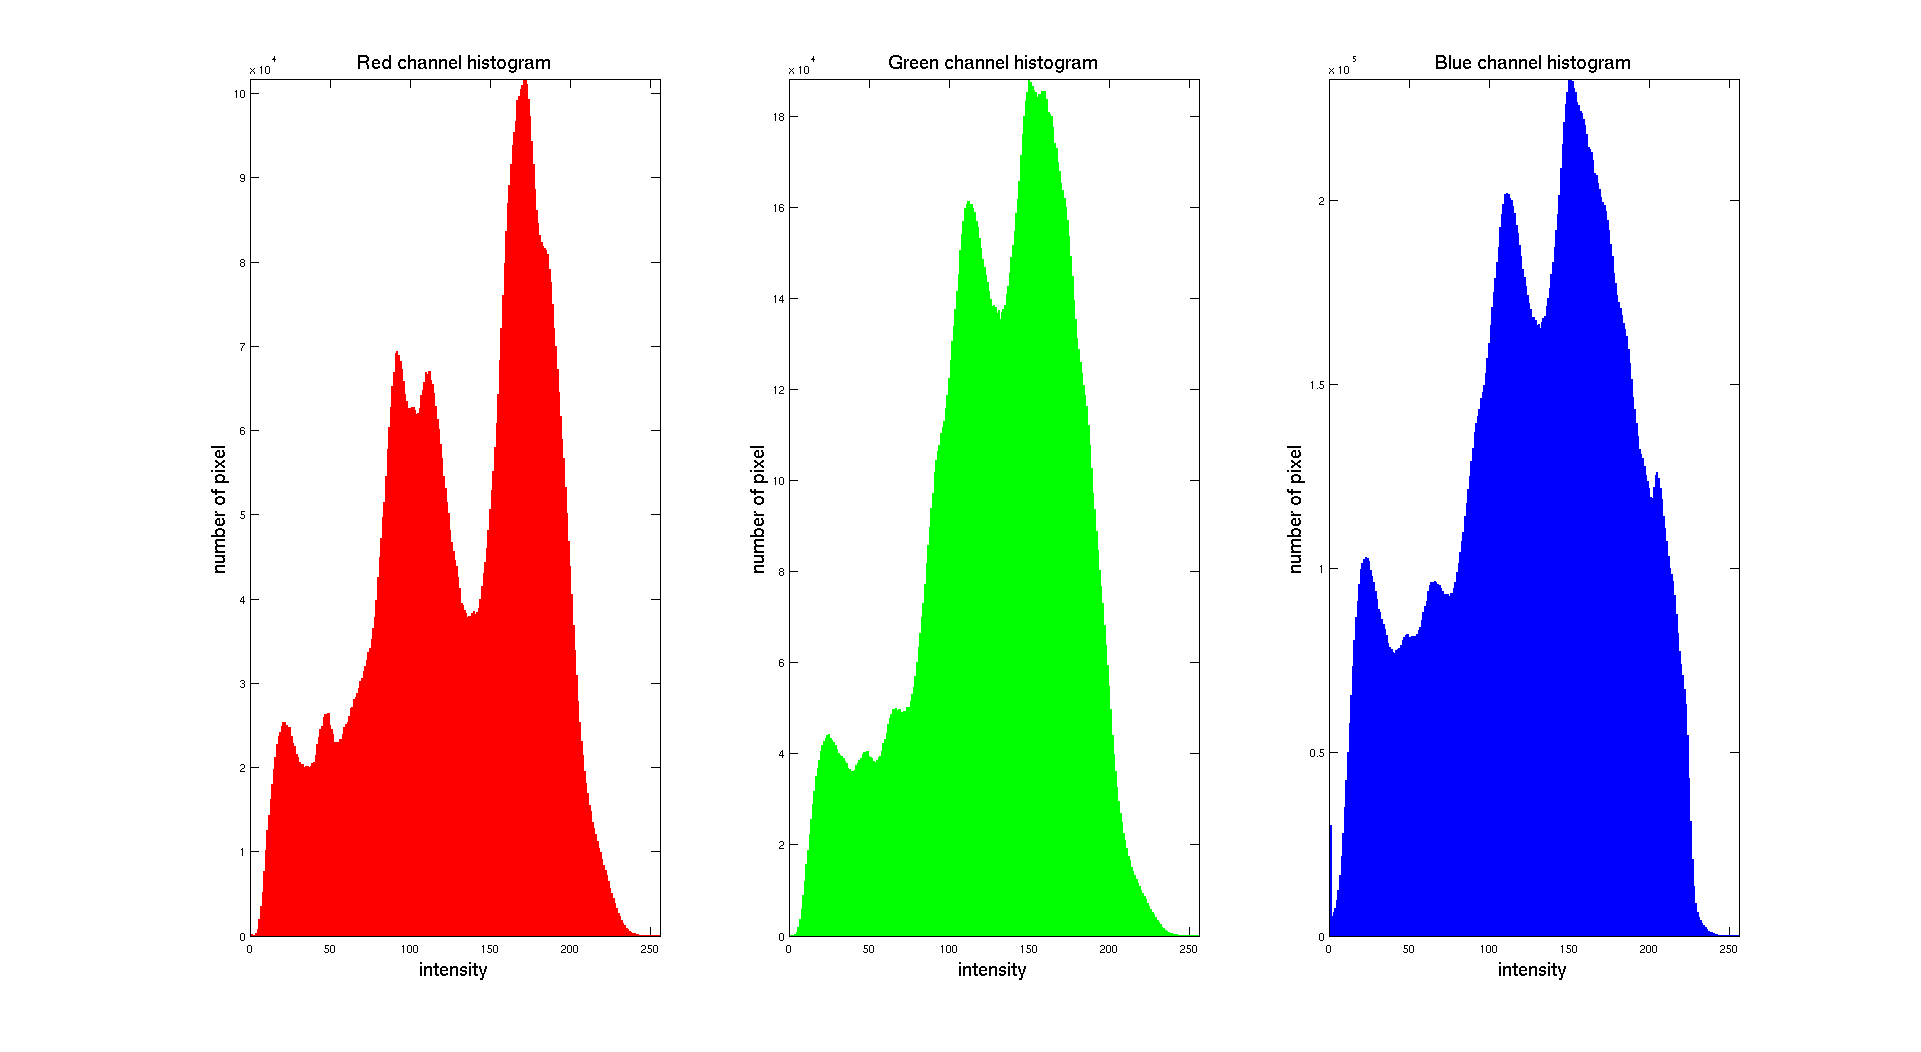
\includegraphics[width=0.6\textwidth, height=0.3\textwidth]{figs/colorhistogram.png}
  \end{figure}

  Color features are chosen as the primary features because of:
  \begin{enumerate}
    \item Highly-invariant to scale and rotation
    \item Highly discriminative as different objects possess different colors
  \end{enumerate}

\end{frame}

\begin{frame}{Caveat 1: Sensitive to illumination}

  \begin{figure}[ht]
      \centering
      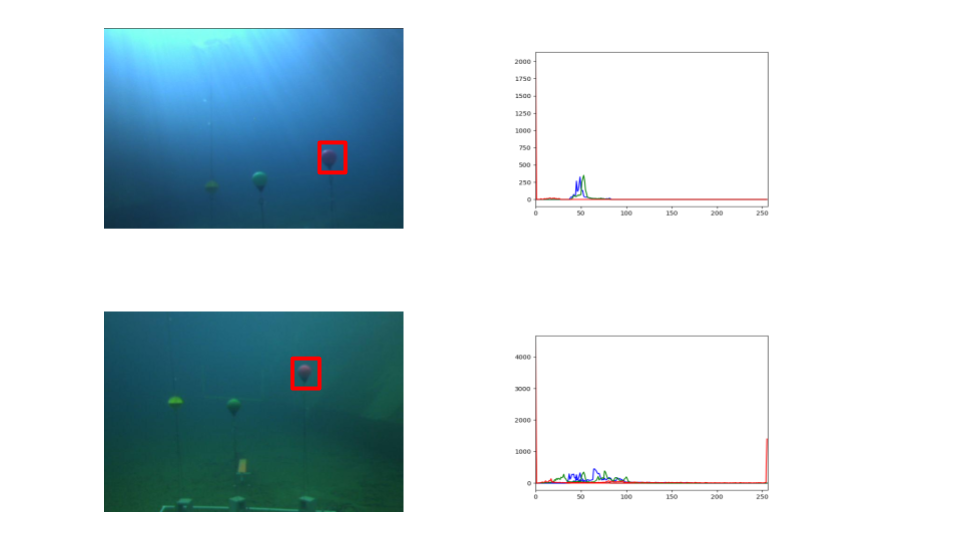
\includegraphics[width=0.6\textwidth, height=0.3\textwidth]{figs/illumsensitive.png}
  \end{figure}

  \begin{enumerate}
    \item Perform color correction to input image before feature extraction
    \item Explore different color spaces that are illumination-invariant
  \end{enumerate}

\end{frame}

\begin{frame}[standout]{}
  Changing color space
\end{frame}

\begin{frame}{rg chromacity}

  \begin{figure}[ht]
      \centering
      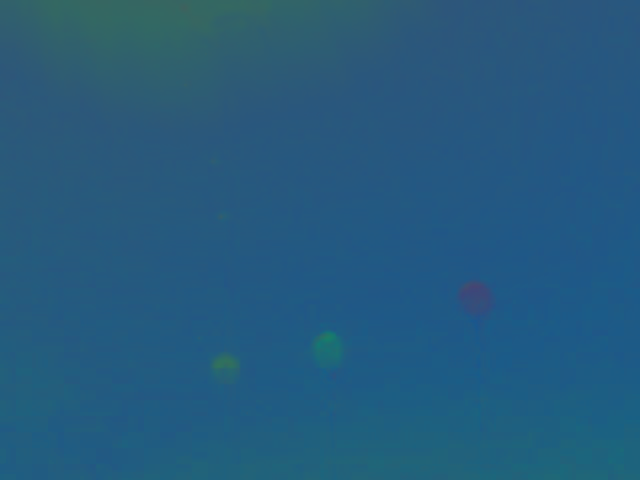
\includegraphics[width=0.5\textwidth, height=0.3\textwidth]{figs/rg.png}
  \end{figure}

  Removes influence of luminance through normalization 
  \[
    r = \frac{R}{R + G + B}, g = \frac{G}{R + G + B}, b = \frac{B}{R + G + B}
  \]
\end{frame}

\begin{frame}{Opponent color space}

  Provides small amount of illumination invariance while maintaning
  discriminative power.
  \[
  \begin{aligned}
    O1 = \frac{R - G}{\sqrt{2}}, O2 = \frac{R + G - 2B}{\sqrt{6}}, O3 = \frac{R +
      G + B}{\sqrt{3}} \\
    W_{o1} = \frac{O1}{O3}, W_{o2} = \frac{O2}{O3}
  \end{aligned}
  \]
\end{frame}

\begin{frame}{Log color ratio}

  Provides complete illumination invariance.
  \[
    L1 = \log{\frac{R}{B}}, L2 = \log{\frac{R}{B}}, L3 = \log{\frac{G}{B}}
  \]
\end{frame}

\begin{frame}{Caveat 2: Insenstive to shape}

  Concatenating shape descriptor with color descriptor. Shape descriptors
  extracted include:

  \begin{enumerate}
    \item Inner shape context
    \item Elliptic Fourier descriptor
    \item Zernike moment
    \item Hu moment
  \end{enumerate}

\end{frame}

%%%%%%%%%%%%%%%%%%%%%%%%%%%%%%%%%%%%%%%%%%%%%%%%%%%%%%%%%%%%%%%%%%%%%%%%%%%%%%%%%%%%%%%%%%%%%%%%%%%%

\section{Object Tracking}

\begin{frame}{Tracking by detection}

  \begin{figure}[ht]
      \centering
      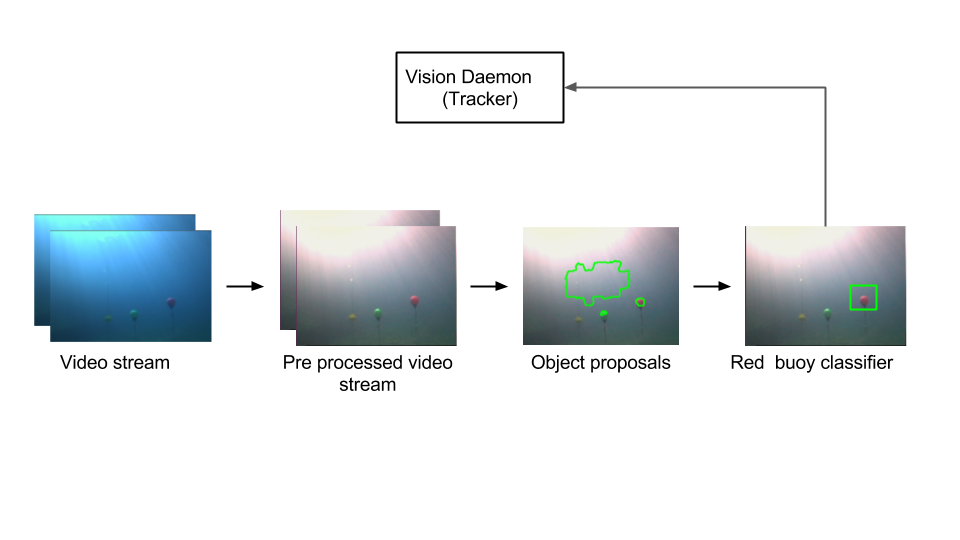
\includegraphics[width=0.8\textwidth, height=0.4\textwidth]{figs/tracker.png}
  \end{figure}

  \begin{enumerate}
    {\small \item Detection is performed on every single incoming frame}
    {\small \item Tracker is reinitialized after losing track for at least 10 frames}
  \end{enumerate}
\end{frame}

\begin{frame}{Scoring mechanism}
  A final score is calculated for each candidate window generated by object
  proposal algorithm.
  \[
    Score_{final} = (1 - \alpha) Score_{classification} + \alpha Score_{prior}
  \]
  The weighted combination of \textit{classification score} and \textit{prior
    score} is used to calculate the final score.
\end{frame}

\begin{frame}{Prior knowledge}
  Non-visual sensor values such as absolute position of the vision obstacle with respect to
  an origin can be used to generate confidence of detection of the object in
  that region.
\end{frame}

\section{Experimental results}

\begin{frame}{Results}

\begin{table}[H]
\resizebox{.8\textwidth}{!}{
\centering
\begin{tabular}{|l|l|l|l|}
\hline
Trackers                           & Accuracy & Robustness & Speed \\ \hline
Baseline                           & 0.21     & 7.23       & 200   \\ \hline
Baseline + preprocessing           & 0.34     & 6.11       & 50    \\ \hline
Baseline + preprocessing +  automl & 0.53     & 2.53       & 50    \\ \hline
MOSSE                              & 0.30     & 8.10       & 100   \\ \hline
KCF                                & 0.35     & 4.91       & 70    \\ \hline
EBT (Edge Box Tracker)             & 0.41     & 3.11       & 43    \\ \hline
\end{tabular}
}
\end{table}

\end{frame}

\begin{frame}[standout]{}
  Q \& A
\end{frame}
%%%%%%%%%%%%%%%%%%%%%%%%%%%%%%%%%%%%%%%%%%%%%%%%%%%%%%%%%%%%%%%%%%%%%%%%%%%%%%%%%%%%%%%%%%%%%%%%%%%%
\end{document}